\documentclass[review]{elsarticle}
% \usepackage[active, tightpage]{preview}

\usepackage{enumitem}
\usepackage{hyperref}
\usepackage{multirow}
\usepackage{pgfplots}
\usepackage{float}
\usepackage{amssymb}
\usepackage{cleveref}
\usepackage[english]{babel}
\usepackage[utf8]{inputenc}
\usepackage[T1]{fontenc}
% \usepackage{changepage}
\usepackage{longtable}
\usepackage{tabularx}
\usepackage{pdfpages}
\usepackage{incgraph,tikz}
% \usepackage[showframe=true]{geometry}
%
\newcommand{\textttt}[1] {\texttt{\footnotesize#1}}
\newcommand{\h} {\hphantom ~ }
% \newcommand{\textttt}[1] {\mbox{\texttt{\footnotesize#1}}}
% \newcommand{\textttt}[1] {
% \begin{verbatim} #1 \end{verbatim}
% }
\pgfplotsset{compat=1.5}
\pgfplotsset
{
	width=0.5\textwidth,
	x tick label style={/pgf/number format/1000 sep=},
  enlarge x limits = 0.0,
  ymajorgrids=true,
	major tick style={draw=none},
  ymin = 0.0,
	every axis/.append style={
		every x tick label/.append style={font=\tiny},
    every y tick label/.append style={font=\tiny},
    every axis label/.append style={font=\small},
    height=37mm,
    width=37mm,
    title style={at={(0.5,0.90)}, font=\normalfont},
    xticklabel style={yshift=4pt}
	}
}

%% `Elsevier LaTeX' style
\bibliographystyle{elsarticle-num}
%
\makeatletter
\def\ps@pprintTitle{%
    \let\@oddhead\@empty
    \let\@evenhead\@empty
    \def\@oddfoot{}%
\let\@evenfoot\@oddfoot}
\makeatother
\begin{document}
%
\begin{frontmatter}
%
\title{Linked Open Social Data for Scientific Benchmarking}
%
\author[pwr]{Renato Fabbri\corref{corresponding}\fnref{kio-url}}
\ead{fabbri@usp.br}
%
\author[pwr]{Osvaldo Novais de Oliveira Junior\fnref{kio-url}}
\ead{chu@ifsc.usp.br}
%
\cortext[corresponding]{Corresponding author}
\address[pwr]{S\~ao Carlos Institute of Physics, S\~ao Paulo
University, Brazil}
%
\fntext[kio-url]{\textit{URL:} \url{http://www.ifsc.usp.br/}}
%
\begin{abstract}
\end{abstract}
%
\begin{keyword}
Big Data, Data Mining, Benchmark Data, Facebook, Twitter, IRC, Email, Complex Networks
%Hierarchy of Clusters \sep HoC \sep Benchmark Dataset \sep Benchmark Data Generator \sep Artificial Data \sep Cluster Analysis \sep Tree Structured Stick Breaking Process \sep TSSB \sep ...
\end{keyword}

\end{frontmatter}
\pdfpageheight 6in
\section{Introduction}
% 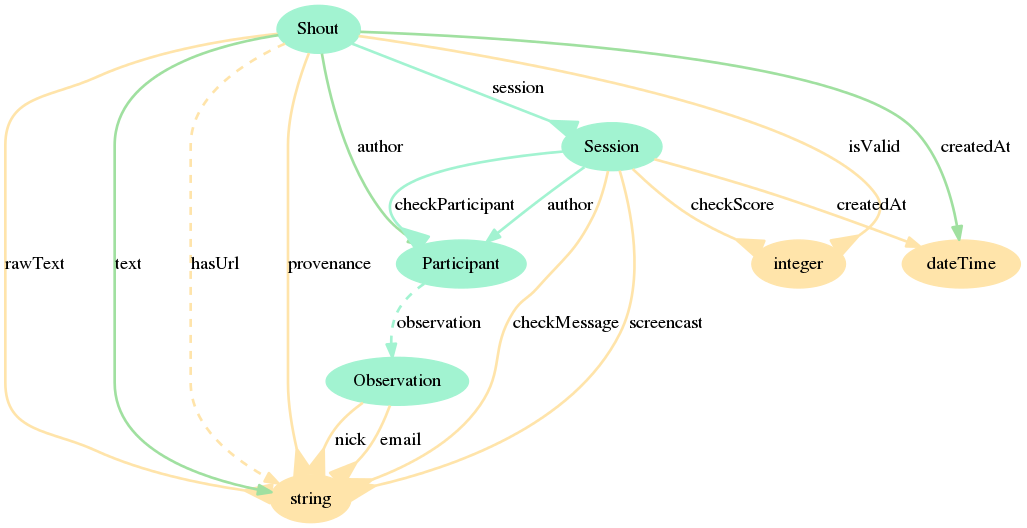
\includepdf{ontologies/aairc.ttl/draw.pdf}
\incgraph[
  overlay={\node[red,below right] at (page.north west) {\Huge Paper sized to picture};}
    paper=graphics
    ]{ontologies/aairc.ttl/draw.png}

\section{Conclusions}
\label{conclusions}
\pdfpageheight 2in
The Linked Open Social Data (LOSD) presented in this article
should be available online in the \url{http://linkedopensocialdata.org}
address in near future to fulfill the purpose of being a common
repertoire in current research.
One should access \url{http://wiki.nosdigitais.teia.org.br/LOSD}
for reaching the address where LOSD is currently reachable.

\section*{References}
%
\bibliography{paper}
%\bibliography{myLastBibfile.bib}
%
\end{document} 
